\section{Introduction}

\begin{definition}[\textit{Syntax analyzer}]
    Syntax analysis, also known as parsing, involves studying the rules that dictate how words or other elements of sentence structure are combined to create grammatically correct sentences.
\end{definition}
The syntax of a language is delineated by a grammar. 
Syntactic analysis entails identifying grammar structures, validating syntactic accuracy, and constructing a derivation tree for the input.
Syntactic analysis processes a stream of terminal symbols, which can be categorized as follows:
\begin{itemize}
    \item \textit{Terminal symbols}: tokens typically generated by the lexer.
    \item \textit{Nonterminal symbols}: produced solely through the reduction of grammar rules.
\end{itemize}

BISON is the primary tool used for generating syntax analyzers, and it seamlessly integrates with FLEX.
Based on the LALR(1) theory, a variation of LR(1), BISON employs a push-down automaton controlled by a directed graph. 
The parsing stack is employed to maintain the parser's state during runtime.

The workflow of FLEX is shown in the following image. 
\begin{figure}[H]
    \centering
    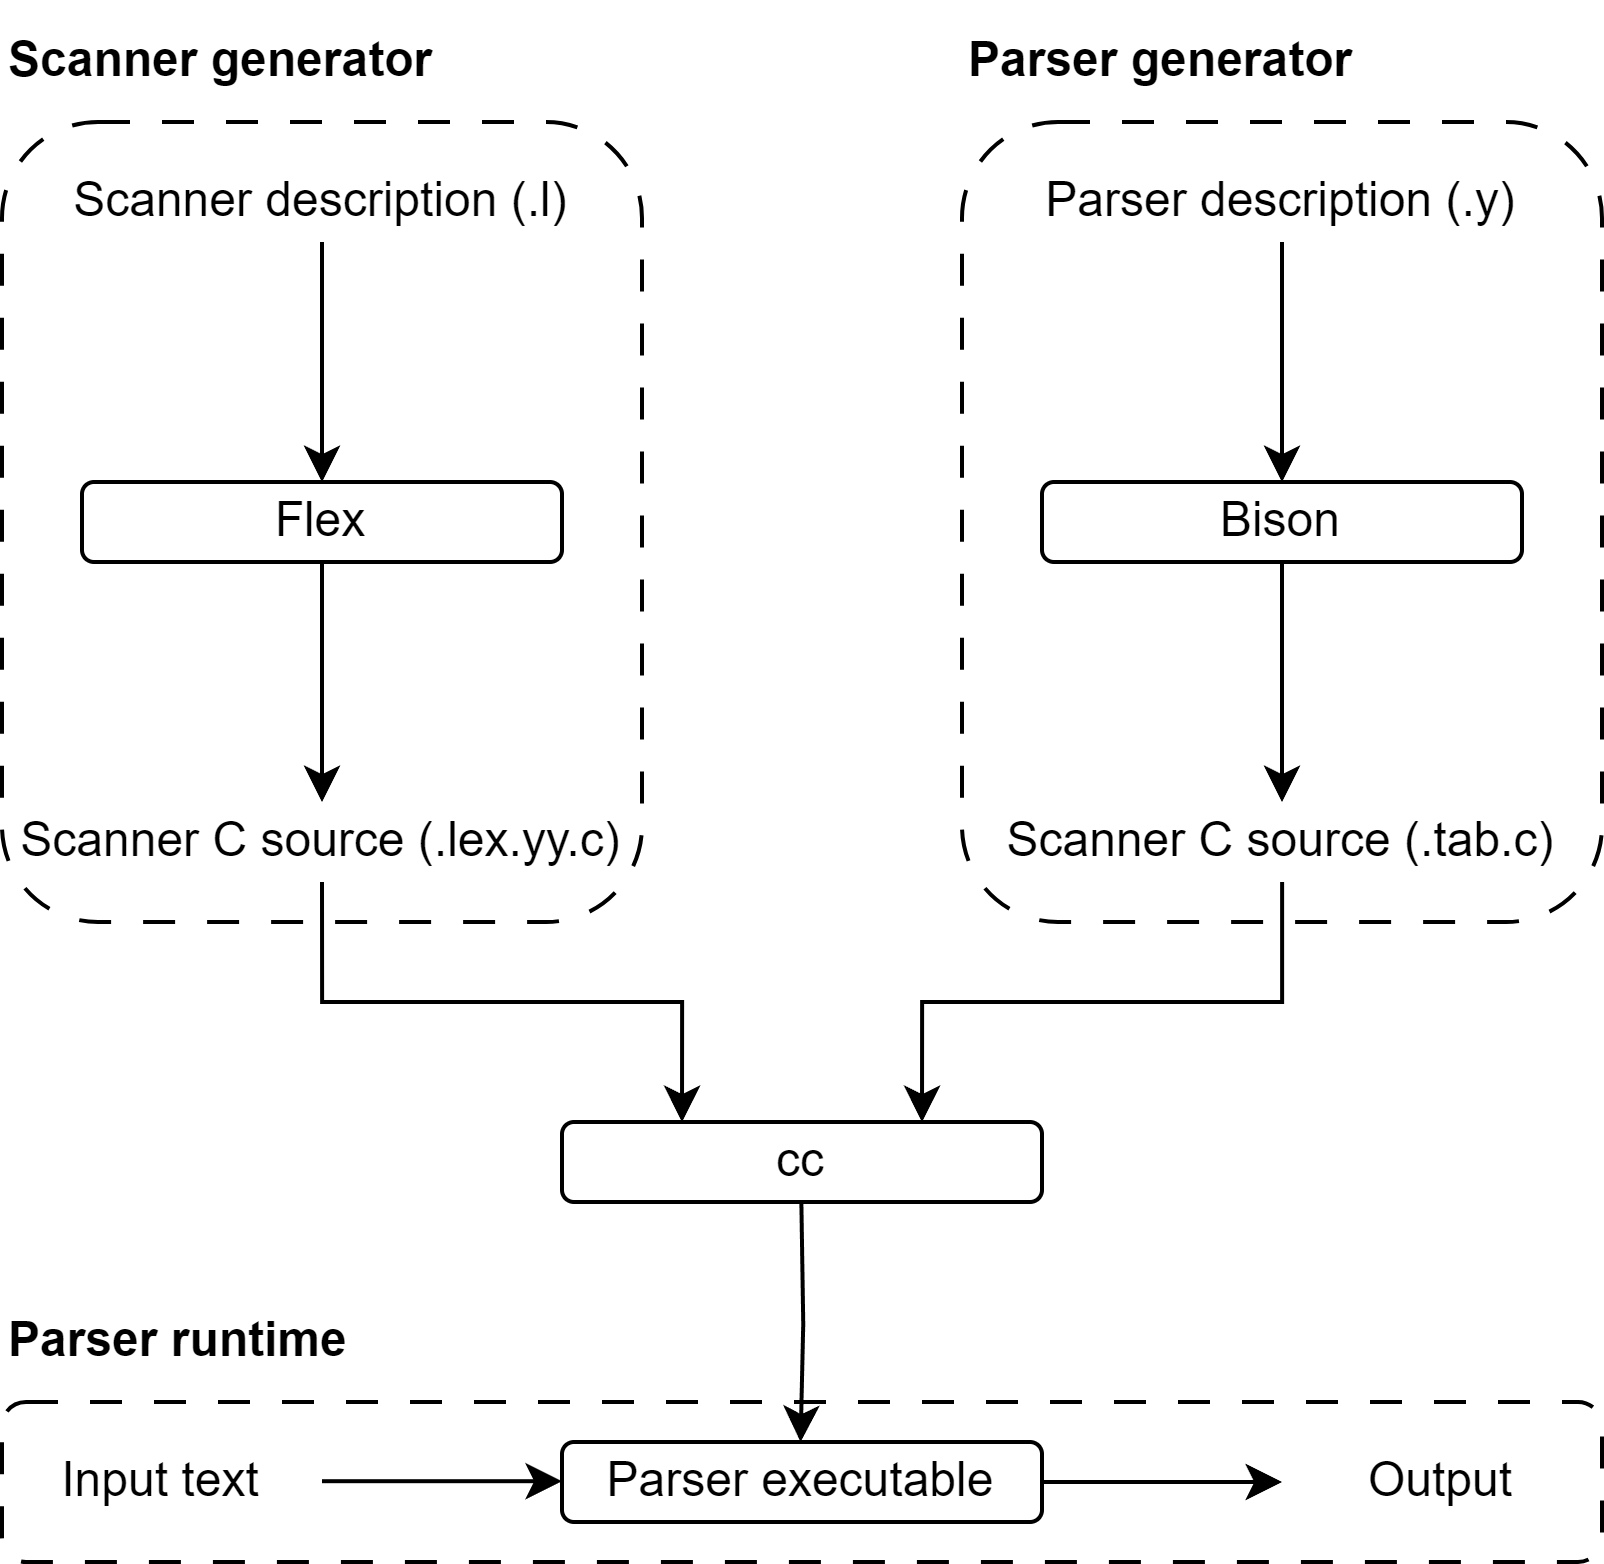
\includegraphics[width=0.39\linewidth]{images/bison.png}
    \caption{BISON workflow}
\end{figure}